% Options for packages loaded elsewhere
\PassOptionsToPackage{unicode}{hyperref}
\PassOptionsToPackage{hyphens}{url}
\PassOptionsToPackage{dvipsnames,svgnames,x11names}{xcolor}
%
\documentclass[
  letterpaper,
  DIV=11,
  numbers=noendperiod]{scrartcl}

\usepackage{amsmath,amssymb}
\usepackage{lmodern}
\usepackage{iftex}
\ifPDFTeX
  \usepackage[T1]{fontenc}
  \usepackage[utf8]{inputenc}
  \usepackage{textcomp} % provide euro and other symbols
\else % if luatex or xetex
  \usepackage{unicode-math}
  \defaultfontfeatures{Scale=MatchLowercase}
  \defaultfontfeatures[\rmfamily]{Ligatures=TeX,Scale=1}
\fi
% Use upquote if available, for straight quotes in verbatim environments
\IfFileExists{upquote.sty}{\usepackage{upquote}}{}
\IfFileExists{microtype.sty}{% use microtype if available
  \usepackage[]{microtype}
  \UseMicrotypeSet[protrusion]{basicmath} % disable protrusion for tt fonts
}{}
\makeatletter
\@ifundefined{KOMAClassName}{% if non-KOMA class
  \IfFileExists{parskip.sty}{%
    \usepackage{parskip}
  }{% else
    \setlength{\parindent}{0pt}
    \setlength{\parskip}{6pt plus 2pt minus 1pt}}
}{% if KOMA class
  \KOMAoptions{parskip=half}}
\makeatother
\usepackage{xcolor}
\setlength{\emergencystretch}{3em} % prevent overfull lines
\setcounter{secnumdepth}{-\maxdimen} % remove section numbering
% Make \paragraph and \subparagraph free-standing
\ifx\paragraph\undefined\else
  \let\oldparagraph\paragraph
  \renewcommand{\paragraph}[1]{\oldparagraph{#1}\mbox{}}
\fi
\ifx\subparagraph\undefined\else
  \let\oldsubparagraph\subparagraph
  \renewcommand{\subparagraph}[1]{\oldsubparagraph{#1}\mbox{}}
\fi

\usepackage{color}
\usepackage{fancyvrb}
\newcommand{\VerbBar}{|}
\newcommand{\VERB}{\Verb[commandchars=\\\{\}]}
\DefineVerbatimEnvironment{Highlighting}{Verbatim}{commandchars=\\\{\}}
% Add ',fontsize=\small' for more characters per line
\usepackage{framed}
\definecolor{shadecolor}{RGB}{241,243,245}
\newenvironment{Shaded}{\begin{snugshade}}{\end{snugshade}}
\newcommand{\AlertTok}[1]{\textcolor[rgb]{0.68,0.00,0.00}{#1}}
\newcommand{\AnnotationTok}[1]{\textcolor[rgb]{0.37,0.37,0.37}{#1}}
\newcommand{\AttributeTok}[1]{\textcolor[rgb]{0.40,0.45,0.13}{#1}}
\newcommand{\BaseNTok}[1]{\textcolor[rgb]{0.68,0.00,0.00}{#1}}
\newcommand{\BuiltInTok}[1]{\textcolor[rgb]{0.00,0.23,0.31}{#1}}
\newcommand{\CharTok}[1]{\textcolor[rgb]{0.13,0.47,0.30}{#1}}
\newcommand{\CommentTok}[1]{\textcolor[rgb]{0.37,0.37,0.37}{#1}}
\newcommand{\CommentVarTok}[1]{\textcolor[rgb]{0.37,0.37,0.37}{\textit{#1}}}
\newcommand{\ConstantTok}[1]{\textcolor[rgb]{0.56,0.35,0.01}{#1}}
\newcommand{\ControlFlowTok}[1]{\textcolor[rgb]{0.00,0.23,0.31}{#1}}
\newcommand{\DataTypeTok}[1]{\textcolor[rgb]{0.68,0.00,0.00}{#1}}
\newcommand{\DecValTok}[1]{\textcolor[rgb]{0.68,0.00,0.00}{#1}}
\newcommand{\DocumentationTok}[1]{\textcolor[rgb]{0.37,0.37,0.37}{\textit{#1}}}
\newcommand{\ErrorTok}[1]{\textcolor[rgb]{0.68,0.00,0.00}{#1}}
\newcommand{\ExtensionTok}[1]{\textcolor[rgb]{0.00,0.23,0.31}{#1}}
\newcommand{\FloatTok}[1]{\textcolor[rgb]{0.68,0.00,0.00}{#1}}
\newcommand{\FunctionTok}[1]{\textcolor[rgb]{0.28,0.35,0.67}{#1}}
\newcommand{\ImportTok}[1]{\textcolor[rgb]{0.00,0.46,0.62}{#1}}
\newcommand{\InformationTok}[1]{\textcolor[rgb]{0.37,0.37,0.37}{#1}}
\newcommand{\KeywordTok}[1]{\textcolor[rgb]{0.00,0.23,0.31}{#1}}
\newcommand{\NormalTok}[1]{\textcolor[rgb]{0.00,0.23,0.31}{#1}}
\newcommand{\OperatorTok}[1]{\textcolor[rgb]{0.37,0.37,0.37}{#1}}
\newcommand{\OtherTok}[1]{\textcolor[rgb]{0.00,0.23,0.31}{#1}}
\newcommand{\PreprocessorTok}[1]{\textcolor[rgb]{0.68,0.00,0.00}{#1}}
\newcommand{\RegionMarkerTok}[1]{\textcolor[rgb]{0.00,0.23,0.31}{#1}}
\newcommand{\SpecialCharTok}[1]{\textcolor[rgb]{0.37,0.37,0.37}{#1}}
\newcommand{\SpecialStringTok}[1]{\textcolor[rgb]{0.13,0.47,0.30}{#1}}
\newcommand{\StringTok}[1]{\textcolor[rgb]{0.13,0.47,0.30}{#1}}
\newcommand{\VariableTok}[1]{\textcolor[rgb]{0.07,0.07,0.07}{#1}}
\newcommand{\VerbatimStringTok}[1]{\textcolor[rgb]{0.13,0.47,0.30}{#1}}
\newcommand{\WarningTok}[1]{\textcolor[rgb]{0.37,0.37,0.37}{\textit{#1}}}

\providecommand{\tightlist}{%
  \setlength{\itemsep}{0pt}\setlength{\parskip}{0pt}}\usepackage{longtable,booktabs,array}
\usepackage{calc} % for calculating minipage widths
% Correct order of tables after \paragraph or \subparagraph
\usepackage{etoolbox}
\makeatletter
\patchcmd\longtable{\par}{\if@noskipsec\mbox{}\fi\par}{}{}
\makeatother
% Allow footnotes in longtable head/foot
\IfFileExists{footnotehyper.sty}{\usepackage{footnotehyper}}{\usepackage{footnote}}
\makesavenoteenv{longtable}
\usepackage{graphicx}
\makeatletter
\def\maxwidth{\ifdim\Gin@nat@width>\linewidth\linewidth\else\Gin@nat@width\fi}
\def\maxheight{\ifdim\Gin@nat@height>\textheight\textheight\else\Gin@nat@height\fi}
\makeatother
% Scale images if necessary, so that they will not overflow the page
% margins by default, and it is still possible to overwrite the defaults
% using explicit options in \includegraphics[width, height, ...]{}
\setkeys{Gin}{width=\maxwidth,height=\maxheight,keepaspectratio}
% Set default figure placement to htbp
\makeatletter
\def\fps@figure{htbp}
\makeatother

\KOMAoption{captions}{tableheading}
\makeatletter
\@ifpackageloaded{tcolorbox}{}{\usepackage[many]{tcolorbox}}
\@ifpackageloaded{fontawesome5}{}{\usepackage{fontawesome5}}
\definecolor{quarto-callout-color}{HTML}{909090}
\definecolor{quarto-callout-note-color}{HTML}{0758E5}
\definecolor{quarto-callout-important-color}{HTML}{CC1914}
\definecolor{quarto-callout-warning-color}{HTML}{EB9113}
\definecolor{quarto-callout-tip-color}{HTML}{00A047}
\definecolor{quarto-callout-caution-color}{HTML}{FC5300}
\definecolor{quarto-callout-color-frame}{HTML}{acacac}
\definecolor{quarto-callout-note-color-frame}{HTML}{4582ec}
\definecolor{quarto-callout-important-color-frame}{HTML}{d9534f}
\definecolor{quarto-callout-warning-color-frame}{HTML}{f0ad4e}
\definecolor{quarto-callout-tip-color-frame}{HTML}{02b875}
\definecolor{quarto-callout-caution-color-frame}{HTML}{fd7e14}
\makeatother
\makeatletter
\makeatother
\makeatletter
\makeatother
\makeatletter
\@ifpackageloaded{caption}{}{\usepackage{caption}}
\AtBeginDocument{%
\ifdefined\contentsname
  \renewcommand*\contentsname{Table of contents}
\else
  \newcommand\contentsname{Table of contents}
\fi
\ifdefined\listfigurename
  \renewcommand*\listfigurename{List of Figures}
\else
  \newcommand\listfigurename{List of Figures}
\fi
\ifdefined\listtablename
  \renewcommand*\listtablename{List of Tables}
\else
  \newcommand\listtablename{List of Tables}
\fi
\ifdefined\figurename
  \renewcommand*\figurename{Figure}
\else
  \newcommand\figurename{Figure}
\fi
\ifdefined\tablename
  \renewcommand*\tablename{Table}
\else
  \newcommand\tablename{Table}
\fi
}
\@ifpackageloaded{float}{}{\usepackage{float}}
\floatstyle{ruled}
\@ifundefined{c@chapter}{\newfloat{codelisting}{h}{lop}}{\newfloat{codelisting}{h}{lop}[chapter]}
\floatname{codelisting}{Listing}
\newcommand*\listoflistings{\listof{codelisting}{List of Listings}}
\makeatother
\makeatletter
\@ifpackageloaded{caption}{}{\usepackage{caption}}
\@ifpackageloaded{subcaption}{}{\usepackage{subcaption}}
\makeatother
\makeatletter
\@ifpackageloaded{tcolorbox}{}{\usepackage[many]{tcolorbox}}
\makeatother
\makeatletter
\@ifundefined{shadecolor}{\definecolor{shadecolor}{rgb}{.97, .97, .97}}
\makeatother
\makeatletter
\makeatother
\ifLuaTeX
  \usepackage{selnolig}  % disable illegal ligatures
\fi
\IfFileExists{bookmark.sty}{\usepackage{bookmark}}{\usepackage{hyperref}}
\IfFileExists{xurl.sty}{\usepackage{xurl}}{} % add URL line breaks if available
\urlstyle{same} % disable monospaced font for URLs
\hypersetup{
  pdftitle={Potential outcomes and Causal Models},
  pdfauthor={Fernando Rios-Avila},
  colorlinks=true,
  linkcolor={blue},
  filecolor={Maroon},
  citecolor={Blue},
  urlcolor={Blue},
  pdfcreator={LaTeX via pandoc}}

\title{Potential outcomes and Causal Models}
\usepackage{etoolbox}
\makeatletter
\providecommand{\subtitle}[1]{% add subtitle to \maketitle
  \apptocmd{\@title}{\par {\large #1 \par}}{}{}
}
\makeatother
\subtitle{What if?}
\author{Fernando Rios-Avila}
\date{}

\begin{document}
\maketitle
\ifdefined\Shaded\renewenvironment{Shaded}{\begin{tcolorbox}[enhanced, breakable, sharp corners, boxrule=0pt, interior hidden, borderline west={3pt}{0pt}{shadecolor}, frame hidden]}{\end{tcolorbox}}\fi

\hypertarget{introduction-what-if}{%
\subsection{Introduction: What if?}\label{introduction-what-if}}

From here on, the whole purpose of the methodologies we will dicusess is
the analysis of causal effects of some:

\begin{quote}
Policy, treatment, experiment, or otherwise event
\end{quote}

But, How is it different from what we did before?

It isn't.

Under Exogeneity assumption \(E(e|X)=0\), one can make causal effect
claims.

\begin{tcolorbox}[enhanced jigsaw, left=2mm, colbacktitle=quarto-callout-important-color!10!white, opacitybacktitle=0.6, leftrule=.75mm, rightrule=.15mm, breakable, coltitle=black, colback=white, opacityback=0, colframe=quarto-callout-important-color-frame, bottomtitle=1mm, toprule=.15mm, arc=.35mm, titlerule=0mm, title=\textcolor{quarto-callout-important-color}{\faExclamation}\hspace{0.5em}{We seek the truth}, toptitle=1mm, bottomrule=.15mm]

How much of the change in outcome is caused by the program alone?

\end{tcolorbox}

But this is not as easy.

\hypertarget{exampleswhere-is-the-challenge}{%
\subsection{Examples\ldots Where is the
challenge?}\label{exampleswhere-is-the-challenge}}

A few examples for Causal effect questions:

\begin{itemize}
\tightlist
\item
  Do minimum wages increase unemployment ?
\item
  Do Conditional cash transfers improve health outcomes in children?
\item
  Do Covid Vaccines help reduce the Spread of Covid?
\end{itemize}

These questions are, however, difficult to answer.

\begin{itemize}
\tightlist
\item
  How do you make sure the ``treatment'' is the Only factor that
  explains the difference in outcome across groups??
\end{itemize}

To do this we need strategies that rule out any other explanation that
could ``take away'' the connection we seek.

\begin{quote}
We need to close \textbf{\emph{all}} back doors, block all
\textbf{alternative} explanations, or nuisanse factors
\end{quote}

\hypertarget{we-need-to-figure-out-what-is-what-we-seek}{%
\section{We need to figure out what is what we
seek}\label{we-need-to-figure-out-what-is-what-we-seek}}

\hypertarget{potential-outcomes}{%
\subsection{Potential Outcomes}\label{potential-outcomes}}

\begin{figure}

{\centering \includegraphics{./po_ci_files/7dhjmq.jpg}

}

\caption{Choice}

\end{figure}

\begin{center}\rule{0.5\linewidth}{0.5pt}\end{center}

In a world of quantum mechanics, multiverses, parallel worlds, and other
infinite number of scenarios, Causal Inference would be extreamly
simple:

\[
\begin{aligned}
Path1 &: Neo \rightarrow RedPill \rightarrow wakesup \rightarrow SavesWorld \\\
Path2 &: Neo \rightarrow BluePill \rightarrow goestoSleep \rightarrow Nothing \ happend
\end{aligned}
\]

Then just compare the outcomes: The read Pill Saved the world.

Thus, treatment effect is simply the difference in the potential
outcomes: \textbf{\emph{Two counterfactuals!}}

This difference captures the TRUE treatment effect. Easy enough\ldots{}

\hypertarget{the-path-not-taken}{%
\subsection{The Path not taken}\label{the-path-not-taken}}

The way we express the \(TE_i\), compares \emph{counterfactuals}. Two
possible States of the world, where an allknowing researcher can
perfectly identify TE.

Unfortunately, the same person cannot take both paths, and we cannot see
both options. A person is either \textbf{Treated} or \textbf{Untreated}.
Thus, the first approach to Casual effects is impossible.

\ldots{}

But it does provide us with a clue of how to go ahead and analyze Causal
effects. We ``simply'' need to estimate the counterfactual!

But before going deeper into how to estimate the counterfactuals And
treatment effects some notation

\hypertarget{potential-outcomes-notation}{%
\subsection{Potential Outcomes:
Notation}\label{potential-outcomes-notation}}

\begin{itemize}
\item
  \(i\) will represent a unit. Person, city, country, school, classroom,
  etc
\item
  \(D\) will indicate the treatment Status of a unit. \(D=1\) means is
  treated, and \(D=0\) is untreated.
\item
  Each unit has two potential outcomes \(Y_i(D=1)\) and \(Y_i(D=0)\)
\item
  All units have only \textbf{one} effective or realized outcome:
  \(Y_i\), which is what we observe, and depends on their treatment
  status:
\end{itemize}

\[Y_i=(1-D_i)*Y_i(0)+D_i*Y_i(1)\]

\begin{itemize}
\item
  Unit Specific causal effect is the difference between potential
  outcomes: \[\delta_i = Y_i(1)-Y_i(0)\]
\item
  \(\pi\) is the proportion of treated units
\end{itemize}

\hypertarget{parameters-of-interest}{%
\subsection{Parameters of Interest}\label{parameters-of-interest}}

Assume we can see the true USCE (unit specific casual effect) for all
units. In addition to their Treatment Status.

There are three parameters one might be interested in analyzing:

\[
\begin{aligned}
ATE &= E(\delta_i) \\
ATT &= E(\delta_i|D_i=1) \\
ATU &= E(\delta_i|D_i=0)
\end{aligned}
\]

In general, this three estimands may tell very different stories.

Lets Put some numbers here

\hypertarget{simulating-effects-stata}{%
\subsection{\texorpdfstring{Simulating effects
\texttt{Stata}}{Simulating effects Stata}}\label{simulating-effects-stata}}

\begin{Shaded}
\begin{Highlighting}[]
\KeywordTok{clear}
\KeywordTok{set} \DecValTok{linesize}\NormalTok{ 255}
\KeywordTok{set} \DecValTok{seed}\NormalTok{ 101}
\KeywordTok{set} \KeywordTok{obs}\NormalTok{ 1000}
\KeywordTok{gen}\NormalTok{ y0 = rnormal(5)}
\KeywordTok{gen}\NormalTok{ t  = rnormal(0.0,0.5)}
\KeywordTok{gen}\NormalTok{ y1 = y0+t}
\NormalTok{** Assume only those with t\textgreater{}0 take treatment}
\KeywordTok{gen}\NormalTok{ trt =(t\textgreater{}0)}
\KeywordTok{gen} \FunctionTok{y}\NormalTok{ = y0 * (1{-}trt) +  y1 * (trt)}
\KeywordTok{format}\NormalTok{ y0 y1 }\FunctionTok{y}\NormalTok{ t \%4.3f }
\OtherTok{list} \KeywordTok{in}\NormalTok{ 1/10, sep(0) }\KeywordTok{clean}
\NormalTok{** For Everyone 100 }\KeywordTok{obs}
\KeywordTok{tabstat}\NormalTok{ t, }\KeywordTok{by}\NormalTok{(trt)}
\end{Highlighting}
\end{Shaded}

\begin{verbatim}
Number of observations (_N) was 0, now 1,000.

          y0        t      y1   trt       y  
  1.   5.254   -0.801   4.453     0   5.254  
  2.   4.997    0.039   5.035     1   5.035  
  3.   2.608   -0.490   2.118     0   2.608  
  4.   6.280   -0.579   5.700     0   6.280  
  5.   5.761    0.090   5.850     1   5.850  
  6.   6.132    0.211   6.342     1   6.342  
  7.   4.928    0.153   5.081     1   5.081  
  8.   4.377   -0.073   4.304     0   4.377  
  9.   3.142    0.427   3.569     1   3.569  
 10.   6.050   -0.332   5.718     0   6.050  

Summary for variables: t
Group variable: trt 

     trt |      Mean
---------+----------
       0 | -.3984745
       1 |  .3748617
---------+----------
   Total | -.0187664
--------------------
\end{verbatim}

\hypertarget{but-there-is-only-1}{%
\subsection{But there is only 1}\label{but-there-is-only-1}}

But, we never see potential outcomes, nor unit specific effects.

The most naive estimator is to just estimate the mean difference in
``post-treatment'' outcome after treatment was in place. But that would
be very biased!

\begin{Shaded}
\begin{Highlighting}[]
\KeywordTok{reg}  \FunctionTok{y}\NormalTok{ trt}
\end{Highlighting}
\end{Shaded}

\begin{verbatim}

      Source |       SS           df       MS      Number of obs   =     1,000
-------------+----------------------------------   F(1, 998)       =     49.49
       Model |  49.4759442         1  49.4759442   Prob > F        =    0.0000
    Residual |  997.714103       998   .99971353   R-squared       =    0.0472
-------------+----------------------------------   Adj R-squared   =    0.0463
       Total |  1047.19005       999  1.04823829   Root MSE        =    .99986
\end{verbatim}

\begin{verbatim}
------------------------------------------------------------------------------
           y | Coefficient  Std. err.      t    P>|t|     [95% conf. interval]
-------------+----------------------------------------------------------------
         trt |
\end{verbatim}

\begin{verbatim}
   .4449359   .0632467     7.03   0.000      .320824    .5690477
       _cons |   4.988793   .0443179   112.57   0.000     4.901826     5.07576
\end{verbatim}

\begin{verbatim}
------------------------------------------------------------------------------
\end{verbatim}

\hypertarget{bias-direction}{%
\subsection{Bias Direction}\label{bias-direction}}

\[
\begin{aligned}
E(Y_i|D_i=1)-E(Y_i|D_i=0) &= ATE  \\
&  +E(Y(0)|D=1)-E(Y(0)|D=0) \\
& +(1-\pi)(ATT-ATU)
\end{aligned}
\]

Intuition: Simple Difference will be biases because

\begin{enumerate}
\def\labelenumi{\arabic{enumi}.}
\item
  There could be a selection bias (one group baseline outcome is
  different from the other)
\item
  Treatment Heterogeneity. Some groups are affected differently from
  others
\end{enumerate}

From these two problems, the second one is easier to handle (either
concentrate on ATT or ATU).

The first one, however, requires using strategies to be able to account
for selection bias.

\hypertarget{independence-assumption}{%
\subsection{Independence assumption}\label{independence-assumption}}

While the Simple mean estimator is most likely to be biased, under
Independence assumption, it may still work:

\[
Y(1),Y(0) \perp D
\]

This means that Treatment Status should NOT depend on the potential
outcomes.

In other words, there shouldnt be any differneces in the potential
outcomes \emph{before} or \emph{after} treatment takes place.

This eliminates the selection bias. And group Heterogeneity.

\[
\begin{aligned}
ATT - ATU &= E(Y|D=1) -  E(Y(0)|D=1) \\
&- E(Y(1)|D=0) -  E(Y|D=0)
\end{aligned}
\]

\hypertarget{sutva}{%
\subsection{SUTVA}\label{sutva}}

\hypertarget{stable-unit-treatment-value-assumption}{%
\subsubsection{Stable Unit Treatment value
assumption}\label{stable-unit-treatment-value-assumption}}

This is a strong assumption that is still required to estimate of
treatment effects.

It assumes that:

\begin{itemize}
\tightlist
\item
  \textbf{Treatment is Homogenous}. Same intensity, quality, type of
  treatment among all treated.
\item
  \textbf{There are no spill overs}. Your Treatment Status effects you
  and you only, and you are only affected by your treatment status. No
  externalities nor Spillovers.
\item
  Also, there are no general equibrium effects
\end{itemize}

This assumptions namely guaranties that when a unit is not treated,
its/his/her outcome will not change.

\hypertarget{narrowing-down-the-problem}{%
\subsection{Narrowing down the
problem}\label{narrowing-down-the-problem}}

\begin{enumerate}
\def\labelenumi{\arabic{enumi}.}
\tightlist
\item
  Individual level effects are impossible to identify. We only observe
  one outcome at a time. (not both)
\item
  It is possible to identify causal effects on groups (treated,
  not-treated, kind-of-treated). But..
\item
  Simple Mean difference will not identify causal effects, unless
  Independence and Sutva assumptions hold
\end{enumerate}

This however, suggests a path. Constructing good counterfactuals can
help idenfiying the Causal effects.

Goal:

\begin{itemize}
\tightlist
\item
  Identify a control/comparison group that is statistically identical to
  the treated group, except for the \textbf{Treatment Status}
\end{itemize}

\hypertarget{the-goal-standard-randomized-control-trials}{%
\subsection{The Goal Standard: Randomized Control
Trials}\label{the-goal-standard-randomized-control-trials}}

\begin{tcolorbox}[enhanced jigsaw, left=2mm, colbacktitle=quarto-callout-important-color!10!white, opacitybacktitle=0.6, leftrule=.75mm, rightrule=.15mm, breakable, coltitle=black, colback=white, opacityback=0, colframe=quarto-callout-important-color-frame, bottomtitle=1mm, toprule=.15mm, arc=.35mm, titlerule=0mm, title=\textcolor{quarto-callout-important-color}{\faExclamation}\hspace{0.5em}{To keep in mind}, toptitle=1mm, bottomrule=.15mm]

Searching for good controls doesnt require having access to perfect
``\emph{clones}''. However, in average, we need groups (T vs UT) that
are very similar to each other.

\end{tcolorbox}

In general, research designed is guided by the rules of program or
treatment assignment on participants.

When researchers have control on the assingment rules, the best approach
is to design a randomized control trial.

In an RCT, randomized assigment, eliminates any selection-bias problems
(although SUTVA remains as an assumption)

\hypertarget{rct-and-selection-problems}{%
\subsection{RCT and Selection
Problems}\label{rct-and-selection-problems}}

Consider the example of the Health Impacts of Hospitals.

\begin{itemize}
\tightlist
\item
  Hospitals (or health care) should improve health of individuals. but
\item
  Only unhealthy people will use Health care services. Selection bias
\item
  Thus It may look that Hospitals Hurt people's health becuase those who
  used it have lower health than those who dont: \[ 
  E(Y|D=1)-E(Y|D=0) = ATT + E(Y(0)|D=1)-E(Y(0)|D=0)
  \]
\end{itemize}

So even if Health services help those in need (ATT). If the selection
bias is large, Naive estimations may suggest Hospitals are harmful.

This is a problem caused because Treatment(going to the Hospital) is
affected by pre-conditions or potential treatment outcomes.

\begin{center}\rule{0.5\linewidth}{0.5pt}\end{center}

Under Random assigment, and SUTVA, this can be fixed:

\begin{enumerate}
\def\labelenumi{\arabic{enumi}.}
\tightlist
\item
  If assigment is given as a lottery, potential benefits (Treatment
  effects) will not be affected by the lottery.
\item
  Here, ATT will be the same as ATU. which will allow us to estimte ATE
  as: \[
  \begin{aligned}
  ATE &= E(Y|D=1)-E(Y|D=0) \\
   &= E(Y|D=1)-E(Y(0)|D=1) \\
   &= E(Y(1)|D=0)-E(Y|D=0) \\
  \end{aligned}
  \]
\end{enumerate}

\hypertarget{stata-example}{%
\subsection{Stata Example}\label{stata-example}}

\begin{Shaded}
\begin{Highlighting}[]
\KeywordTok{gen}\NormalTok{ trt2=rnormal()\textgreater{}0}
\KeywordTok{gen}\NormalTok{ yrct = y0 * (1{-}trt2) +  y1 * (trt2)}
\KeywordTok{tabstat}\NormalTok{ t y0 y1 yrct, }\KeywordTok{by}\NormalTok{(trt2)}
\KeywordTok{reg}\NormalTok{ yrct trt2}
\end{Highlighting}
\end{Shaded}

\begin{verbatim}

Summary statistics: Mean
Group variable: trt2 

    trt2 |         t        y0        y1      yrct
---------+----------------------------------------
       0 | -.0097507  5.061626  5.051875  5.061626
       1 |  -.027891  4.984309  4.956418  4.956418
---------+----------------------------------------
   Total | -.0187664  5.023199  5.004433  5.009338
--------------------------------------------------

      Source |       SS           df       MS      Number of obs   =     1,000
-------------+----------------------------------   F(1, 998)       =      2.64
       Model |  2.76706003         1  2.76706003   Prob > F        =    0.1046
    Residual |  1046.22695       998   1.0483236   R-squared       =    0.0026
-------------+----------------------------------   Adj R-squared   =    0.0016
       Total |  1048.99401       999  1.05004406   Root MSE        =    1.0239

------------------------------------------------------------------------------
        yrct | Coefficient  Std. err.      t    P>|t|     [95% conf. interval]
-------------+----------------------------------------------------------------
        trt2 |  -.1052076   .0647568    -1.62   0.105    -.2322827    .0218675
       _cons |   5.061626   .0456524   110.87   0.000      4.97204    5.151212
------------------------------------------------------------------------------
\end{verbatim}

\hypertarget{internal-vs-external-validity}{%
\subsection{Internal vs External
Validity}\label{internal-vs-external-validity}}

RCTs are not the only strategy that allows you to control the Rules of
Treatment. In \textbf{\emph{Experimental Economics}} this is done quite
often

\begin{quote}
you select your sample (of students), and randomly assigned treatments
of interest (Experimental design).
\end{quote}

There are, however, further considerations to be taken:

\begin{tcolorbox}[enhanced jigsaw, left=2mm, colbacktitle=quarto-callout-important-color!10!white, opacitybacktitle=0.6, leftrule=.75mm, rightrule=.15mm, breakable, coltitle=black, colback=white, opacityback=0, colframe=quarto-callout-important-color-frame, bottomtitle=1mm, toprule=.15mm, arc=.35mm, titlerule=0mm, title=\textcolor{quarto-callout-important-color}{\faExclamation}\hspace{0.5em}{Internal Validity}, toptitle=1mm, bottomrule=.15mm]

The estimated Impact is net of all other confunding factors (Random
assigment)

\end{tcolorbox}

\begin{tcolorbox}[enhanced jigsaw, left=2mm, colbacktitle=quarto-callout-important-color!10!white, opacitybacktitle=0.6, leftrule=.75mm, rightrule=.15mm, breakable, coltitle=black, colback=white, opacityback=0, colframe=quarto-callout-important-color-frame, bottomtitle=1mm, toprule=.15mm, arc=.35mm, titlerule=0mm, title=\textcolor{quarto-callout-important-color}{\faExclamation}\hspace{0.5em}{External Validity}, toptitle=1mm, bottomrule=.15mm]

The estimated impact can be generalized to the population in general.
(Random Sample)

\end{tcolorbox}

\begin{tcolorbox}[enhanced jigsaw, left=2mm, colbacktitle=quarto-callout-important-color!10!white, opacitybacktitle=0.6, leftrule=.75mm, rightrule=.15mm, breakable, coltitle=black, colback=white, opacityback=0, colframe=quarto-callout-important-color-frame, bottomtitle=1mm, toprule=.15mm, arc=.35mm, titlerule=0mm, title=\textcolor{quarto-callout-important-color}{\faExclamation}\hspace{0.5em}{How to Randomize}, toptitle=1mm, bottomrule=.15mm]

Depends mostly on how reasonable is to mantain SUTVA assumption

\end{tcolorbox}

\hypertarget{examples}{%
\subsection{Examples}\label{examples}}

\begin{tcolorbox}[enhanced jigsaw, left=2mm, colbacktitle=quarto-callout-note-color!10!white, opacitybacktitle=0.6, leftrule=.75mm, rightrule=.15mm, breakable, coltitle=black, colback=white, opacityback=0, colframe=quarto-callout-note-color-frame, bottomtitle=1mm, toprule=.15mm, arc=.35mm, titlerule=0mm, title=\textcolor{quarto-callout-note-color}{\faInfo}\hspace{0.5em}{CCT and Education in Mexico}, toptitle=1mm, bottomrule=.15mm]

Progresa/Prospera is a CCT program for poor mothers based on children
school enrollment to suport education attainment.

Eligibility was based on Census data on Poverty levels and Baseline Data
collection. But during phase-in period, only 2/3 if localities were
selected to receive the Transfer

\end{tcolorbox}

\begin{tcolorbox}[enhanced jigsaw, left=2mm, colbacktitle=quarto-callout-note-color!10!white, opacitybacktitle=0.6, leftrule=.75mm, rightrule=.15mm, breakable, coltitle=black, colback=white, opacityback=0, colframe=quarto-callout-note-color-frame, bottomtitle=1mm, toprule=.15mm, arc=.35mm, titlerule=0mm, title=\textcolor{quarto-callout-note-color}{\faInfo}\hspace{0.5em}{Water and Sanitation Intervention in Bolivia}, toptitle=1mm, bottomrule=.15mm]

In 2012 IADB and Bolivian Goverment implemented a random assigment of
water/sanitation interventions in Small Rural Communities.

From 369 eliginle communities, 182 were selected at random for the
program implementation, via public lotteries, constraining on Community
Size

\end{tcolorbox}

\hypertarget{how-to-analyze-the-data}{%
\subsection{How to Analyze the Data}\label{how-to-analyze-the-data}}

\begin{enumerate}
\def\labelenumi{\arabic{enumi}.}
\tightlist
\item
  \textbf{Verify Data Balance}: Even if treatment was assigned at
  random, it is important to verify of groups remain comparable. (Thus
  avoid compossition effects)
\item
  \textbf{Mean Difference}: Because of Random Assigment, one could use
  simple mean differences to estimate ATE
\item
  \textbf{Consider using controls}: Under RA, controls will not affect
  the outcome, but may improve precision:
  \(y_i = \alpha_0 + \tau D_i + x_i\beta + \varepsilon_i\).

  \begin{itemize}
  \tightlist
  \item
    But controls should not be affected by the treatment itself (thus
    should be pre-treatment)
  \end{itemize}
\item
  May consider \textbf{falsification} tests
\item
  And Other Robustness test: Outliers, or distributional impacts may be
  of interest
\end{enumerate}

\hypertarget{example}{%
\section{Example}\label{example}}

School subsidies for the poor:

Evaluating the Mexican Progresa poverty program

Paul Schultz (2004)

\hypertarget{background}{%
\subsection{Background}\label{background}}

Progresa is a Cash Transfer Program designed to increase School
Enrollment among the poor, minimizing desincentives to work.

This program provided Grants to families whos children attended school
for atleast 85\% of the school year, covering between 50/75\% of school
cost.

While there were 495 localities that were eligible to benefit from the
program, only 314 were \textbf{randomly} selected to start reciving
resources for the first 2 years. With the unselected localities being
treated a couple of years later.

\begin{quote}
The program continued beyond the original scope of the policy, now its
known as Progresa/Oportunidades
\end{quote}

\hypertarget{method}{%
\subsection{Method}\label{method}}

Goal. Estimate the impact of Progresa (P) on Enrollment (S) \[
S_i = a_0 +a_1 P_i + a_2 E_i + a_3 P_iE_i + \delta Enrolled_c + \beta X + e_i
\]

\(P_i=1\) if the comunity is eligible

\(E_i=1\) if the child is Poor

\$P\_i * E\_i \$ the impact on Poor Chilren in eligible communities.

Model can be estimated Separately (5 years), or using pooled data

This is a kind of DIDID model. However, we could consider it as a simple
mean comparison between those Effectively treated and those untreated.

\hypertarget{differences-in-characteristics}{%
\subsection{Differences in
Characteristics}\label{differences-in-characteristics}}

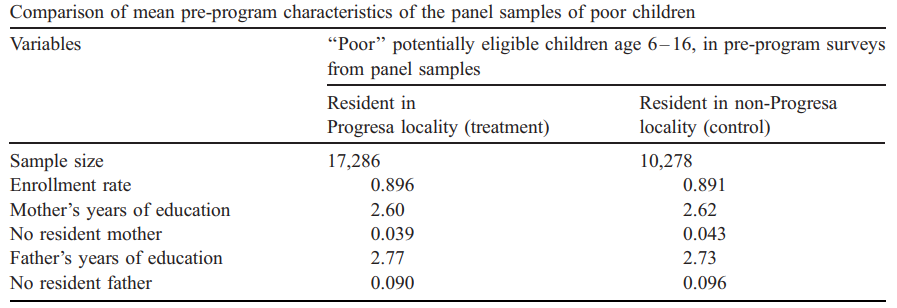
\includegraphics{./po_ci_files/fig3.png}
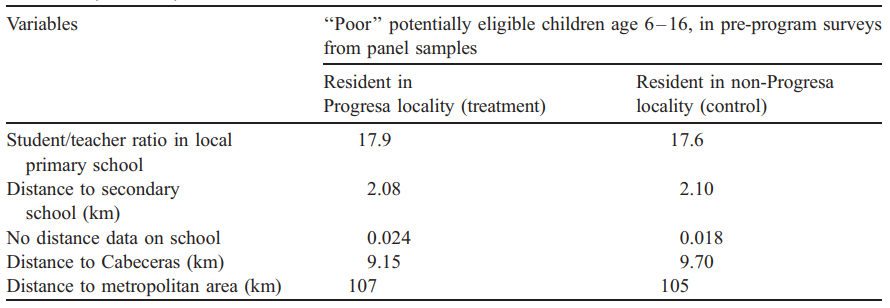
\includegraphics{./po_ci_files/fig4.png}

\hypertarget{raw-differences}{%
\subsection{Raw Differences}\label{raw-differences}}

\begin{figure}

{\centering 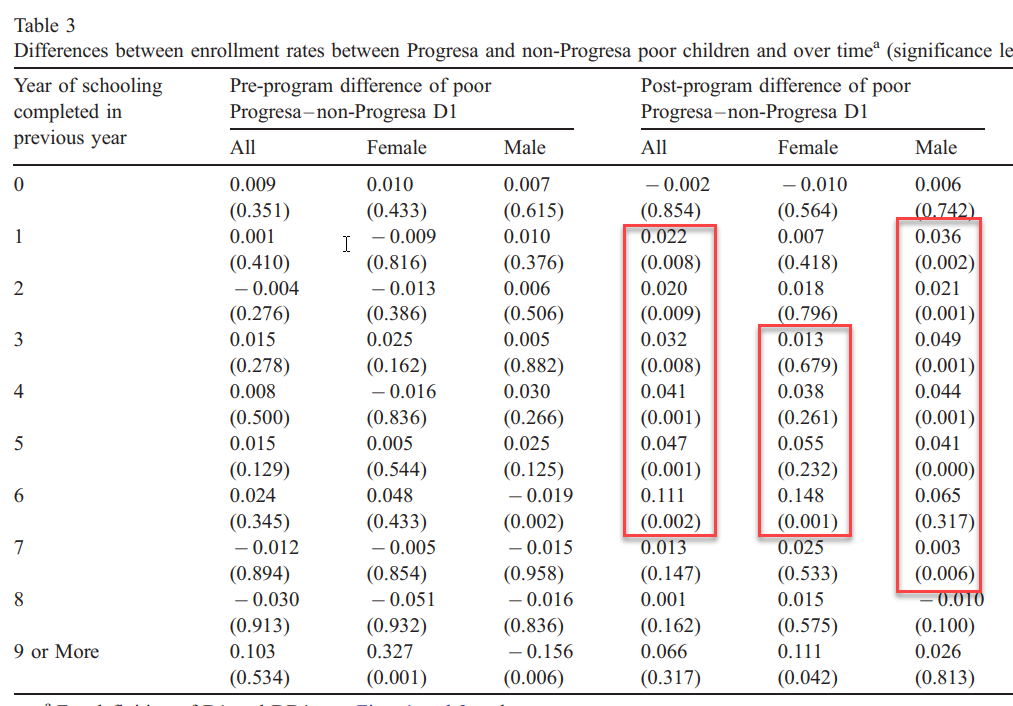
\includegraphics{./po_ci_files/fig1.png}

}

\caption{Poor HH}

\end{figure}

\begin{center}\rule{0.5\linewidth}{0.5pt}\end{center}

\begin{figure}

{\centering 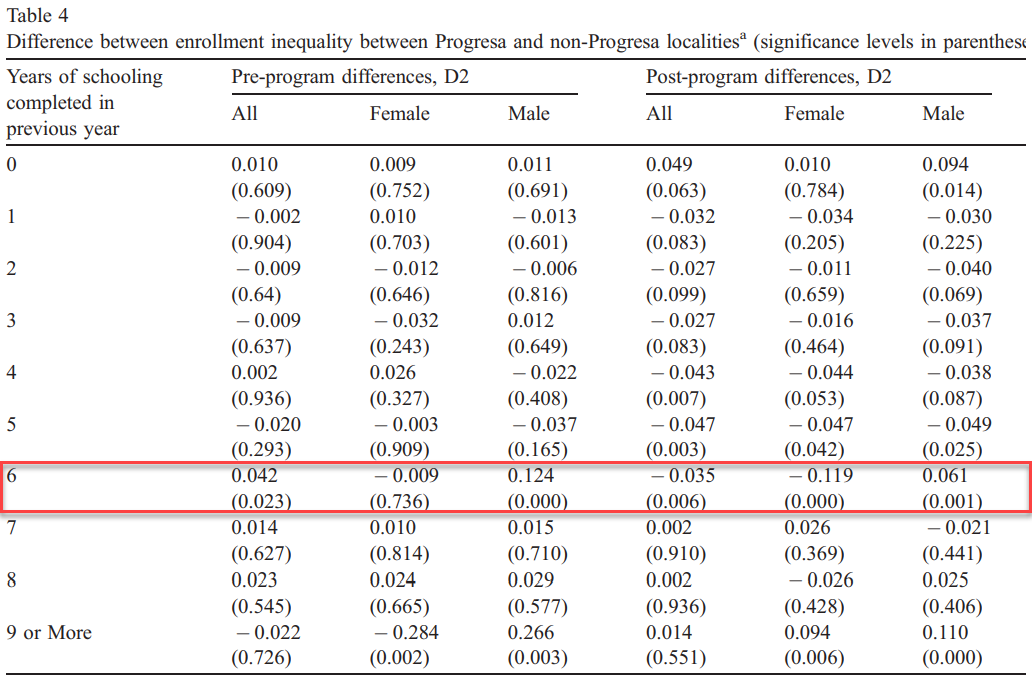
\includegraphics{./po_ci_files/fig2.png}

}

\caption{Non Poor HH}

\end{figure}

\hypertarget{with-controls}{%
\subsection{With Controls}\label{with-controls}}

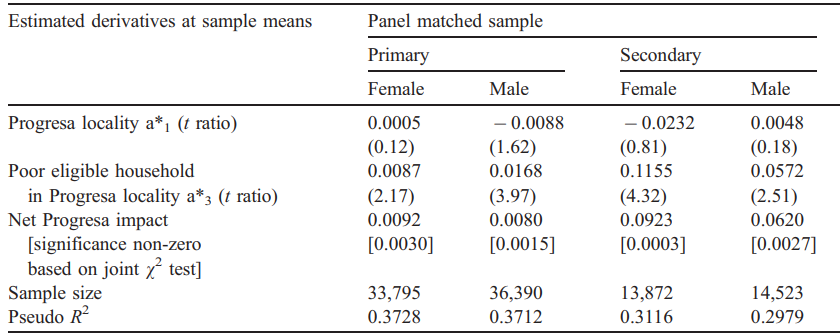
\includegraphics{./po_ci_files/fig6.png}

\hypertarget{other-outcomes}{%
\subsection{Other Outcomes}\label{other-outcomes}}

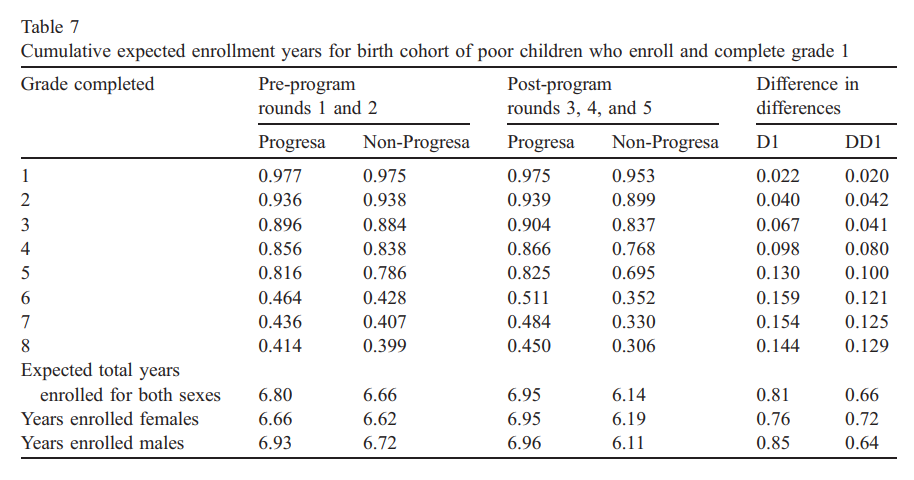
\includegraphics{./po_ci_files/fig5.png}

\hypertarget{next-class-matching-and-weighting}{%
\section{Next Class: Matching and
Weighting}\label{next-class-matching-and-weighting}}



\end{document}
